%%%%%%%%%%%%%%%%%%%%%%%%%%%%%%%%%%%%%%%%%%%%%%%%%%%%%%%%%%%%%%%%%%%%%%
% How to use writeLaTeX: 
%
% You edit the source code here on the left, and the preview on the
% right shows you the result within a few seconds.
%
% Bookmark this page and share the URL with your co-authors. They can
% edit at the same time!
%
% You can upload figures, bibliographies, custom classes and
% styles using the files menu.
%
%%%%%%%%%%%%%%%%%%%%%%%%%%%%%%%%%%%%%%%%%%%%%%%%%%%%%%%%%%%%%%%%%%%%%%

\documentclass[12pt]{article}
\usepackage{adjustbox}
\usepackage{sbc-template}
\usepackage{todonotes}
\usepackage{graphicx,url}
\usepackage{amsmath}
\usepackage{multirow}
\usepackage[utf8]{inputenc}  
\usepackage{babel}
\usepackage[T1]{fontenc}
\usepackage{xspace}
\usepackage{url}
\usepackage{graphicx}
\usepackage{subfig}
%----------
\usepackage{unicode-math}
\usepackage{babel}
\babeltags{br = brazil, en = english}
\usepackage[T1]{fontenc}
\usepackage{xspace}
\usepackage{url}
\usepackage{lipsum} 
%\setmathfont{xits-math.otf}
\usepackage{enumerate}
%\setmathfont[math-style=upright,range={`e,`i}]{xits-math.otf}

%--------------
\sloppy

\title{Calculo Numérico\\Trabalho\_4}


\author{Prof. Dra. Larissa de Freitas \inst{1},\\Guilherme de Souza\inst{1}}

\begin{document} 

\maketitle
\br
%\section{Funções}
%\begin{eqnarray}
%$\lambda x: 5x^{3} - 2x^{2} + 8x - 10$\\
%$\lambda x: 2x^{3} + 5x^{2} + \sin x - 30$\\
%$\lambda x: e^{-x2}\cos x$\\
%    $\lambda x: (x+1)(x-1)(x-3)^{5}\\
%    $\lambda x: (x+2)^{3}\sqrt{x^{2}+1}$
%\end{eqnarray}

\section{Métodos implementados}
\begin{itemize}
  \item Trapezio;
  \item 1/3 de Simpsom;
  \item 3/8 de Simpsom ;
  \item Euler ???;
  \item Runge-Kutta 2a Ordem;
  \item Runge-Kutta 4a Ordem;
  \item Adams;
\end{itemize}

Para execução de tais métodos como, \textbf{Trapezio, 1/3 de Simpsom e 3/8 de Simpsom} foram aplicados na lista de exercícios 11\footnote{Disponivel no AVA:\url{https://ava.ufpel.edu.br/pre/pluginfile.php/318455/mod_resource/content/1/ListaDeExercicios11.pdf}}. Os métodos de \textbf{Runge-Kutta 2a ordem}, \textbf{4a ordem} e \textbf{Adams} utilizou-se a lista de exercícios 12\footnote{Disponivel no AVA:\url{https://ava.ufpel.edu.br/pre/pluginfile.php/320366/mod_resource/content/2/ListaDeExercicios12.pdf}}.


\section{Método do Trapezio}

%---------------------------------------------------------------------------------------------------
% Resultados 
%---------------------------------------------------------------------------------------------------
\begin{itemize}
    \item \textbf{(A)} Trapezio: 31.365285650063754
\end{itemize}

\begin{table}[ht]
\centering
\begin{tabular}{|lllll|}
-1.08268227 & -0.73575888 & 0.0 & 5.43656366 & 59.11244879
\end{tabular}
    \caption{Função utlizando a regra do trapezio no exercício A da lista 11}
\end{table}


\begin{itemize}
    \item \textbf{(B)} Trapezio: 0.7842407666178157
\end{itemize}

\begin{table}[ht]
\centering
\begin{tabular}{|lllllll|}
  0.5 & 0.97297297 & 0.9 & 0.8 & 0.69230769 & 0.59016393 & 0.25
\end{tabular}
    \caption{Função utlizando a regra do trapezio no exercício B da lista 11}
\end{table}


\begin{itemize}
    \item \textbf{(C)} Trapezio: 0.10486282062502501
\end{itemize}

\begin{table}[ht]
\centering
\begin{tabular}{|lllllll|}
  0.0 & 0.20999043 & 0.69856645 & 1.08060461 & 0.83640026 & -0.53179749 & -1.66458735
\end{tabular}
    \caption{Função utlizando a regra do trapezio no exercício C da lista 11}
\end{table}


\begin{itemize}
    \item \textbf{(D)} Trapezio: -13.575979391799388
\end{itemize}
\begin{table}[ht]
\centering
\begin{tabular}{|lllllllll|}
0.0 & 2.24766465 & 5.42294499 & 6.97416428 & 2.08548731 & -13.92608463 & -39.26843454 & -56.88800791 & -15.25556929
\end{tabular}
    \caption{Função utlizando a regra do trapezio no exercício D da lista 11}
\end{table}


\begin{itemize}
    \item \textbf{(E)} Trapezio: 0.5196110146984233
\end{itemize}
\begin{table}[ht]
\centering
\begin{tabular}{|lllllllll|}
  0.4  & 0.71910112  & 0.64 & 0.56637168 & 0.5 & 0.44137931 & 0.3902439 & 0.34594595 & 0.15384615
\end{tabular}
    \caption{Função utlizando a regra do trapezio no exercício E da lista 11}
\end{table}


\section{1/3 de Simpsom}


%---------------------------------------------------------------------------------------------------
% Resultados
%---------------------------------------------------------------------------------------------------
\begin{itemize}
    \item \textbf{(A)} 1/3 de Simpsom: 22.231872397453277
\end{itemize}
\begin{table}[ht]
\centering
\begin{tabular}{|lllll|}
 -1.08268227 & -1.47151776 & -0.73575888 & 10.87312731 & 10.87312731
\end{tabular}
    \caption{Função utlizando a regra do trapezio no exercício A da lista 11}
\end{table}


\begin{itemize}
    \item \textbf{(B)} 1/3 de Simpsom: 0.8054718653079309
\end{itemize}
\begin{table}[ht]
\centering
\begin{tabular}{|lllllll|}
     0.5 & 1.94594595 &  0.97297297 & 1.6 & 0.8 & 1.18032787 & 0.29508197
\end{tabular}
    \caption{Função utlizando a regra do trapezio no exercício B da lista 11}
\end{table}


\begin{itemize}
    \item \textbf{(C)} 1/3 de Simpsom: 0.12706697873621364
\end{itemize}
\begin{table}[ht]
\centering
\begin{tabular}{|lllllll|}
     0.0 & 0.41998087 &  0.20999043 & 2.16120922 & 1.08060461 & -1.06359498 & -0.26589874
\end{tabular}
    \caption{Função utlizando a regra do trapezio no exercício C da lista 11}
\end{table}


\begin{itemize}
    \item \textbf{(D)} 1/3 de Simpsom: -11.92869601630686
\end{itemize}
\begin{table}[ht]
\centering
\begin{tabular}{|lllllllll|}
    0.0 & 4.49532929  &  2.24766465 & 13.94832857 & 6.97416428 & -27.85216926 & -13.92608463 & -113.77601581  & -28.44400395
\end{tabular}
    \caption{Função utlizando a regra do trapezio no exercício D da lista 11}
\end{table}

\section{Cholesky}

Seguindo a mesma idéia em ganho de eficiência como no método anterior apresentado, o método de cholesky tem por objetivo decompor A em G$G^{T}$ desde que sua matriz seja positiva definida. Assim teremos uma matriz triangular inferior e sua matriz adjunta. Esse método é comumente usado para simulações de Monte Carlo, ja demonstrado ser duas vezes mais eficiênte que a fatoração LU. Os resultados podem ser visto a seguir, obervando as Tabelas 22 a 30.
%--------------------------------------------------------------------------------------------------------------------------------
%    MATRIZ 1
%--------------------------------------------------------------------------------------------------------------------------------

\begin{table}[!ht]
  \begin{minipage}[b]{.36\linewidth}

    \centering
    \begin{tabular}{|c c c|}
        3                 &         0                   &           0    \\
        -2          &         5                   &          0  \\
        1           &         -1           &          4    \\
    \end{tabular}
    \caption{Matriz G 1}
    \label{tab:dir}


  \end{minipage}\hfill
  \begin{minipage}[b]{.46\linewidth}

    \centering
    \begin{tabular}{|c|}
        -1\\
        0\\
        2\\
    \end{tabular}
    \caption{Resolução Matriz 1}
    \label{tab:dir}
  \end{minipage}\hfill
  \begin{minipage}[b]{.36\linewidth}

    \centering
    \begin{tabular}{|c c c|}
        3                 &         -2       &           1  \\
        0          &         5          &          -1       \\
        0           &         0               &          4  \\
    \end{tabular}
      \caption{Matriz GT 1}
    \label{tab:esq}
  \end{minipage}

\end{table}


%---------------------------------------------------------------------------------------------------
% MATRIZ 2
%---------------------------------------------------------------------------------------------------
\begin{table}[!ht]
  \begin{minipage}[b]{.36\linewidth}

    \centering
    \begin{tabular}{|c c c c|}
        2           &         0                   &           0             &   0     \\
        -1          &         1.41421            &          0               &   0     \\
        2           &         0.70711           &          3.08221                &   0 \\
        5          &         -1.41422            &           0          &   1.8918  \\
    \end{tabular}
    \caption{Matriz G 2}
    \label{tab:dir}


  \end{minipage}\hfill
  \begin{minipage}[b]{.46\linewidth}

    \centering
    \begin{tabular}{|c|}
        3\\
        1\\
        -0\\
        -1\\
    \end{tabular}
    \caption{Resolução Matriz 2}
    \label{tab:dir}
  \end{minipage}\hfill
  \begin{minipage}[b]{.36\linewidth}

    \centering
    \begin{tabular}{|c c c c|}
        2                 &         -1       &           2             &   5    \\
        0          &        1.41421          &          0.70711        &   -1.41422      \\
        0           &         0               &         3.08221      &   0.64889     \\
        0          &         0                &           0             &   1.8918    \\
    \end{tabular}
      \caption{Matriz GT 2}
    \label{tab:esq}
  \end{minipage}

\end{table}



%---------------------------------------------------------------------------------------------------
% MATRIZ 3
%---------------------------------------------------------------------------------------------------
\begin{table}[!ht]
  \begin{minipage}[b]{.36\linewidth}

    \centering
    \begin{tabular}{|c c c c c|}
        1&         0 &           0             &   0     &   0   \\
        2&         1&          0               &   0     &   0   \\
        -3&         5&          4                &   0     &   0   \\
        0&         1&           -1          &   2    &     0  \\
        3&         -2&           0           &   1    &     5\\
    \end{tabular}
    \caption{Matriz G 3}
    \label{tab:dir}


  \end{minipage}\hfill
  \begin{minipage}[b]{.46\linewidth}

    \centering
    \begin{tabular}{|c|}
        -2\\
        8\\
        -1\\
        4\\
        0\\
    \end{tabular}
    \caption{Resolução Matriz 3}
    \label{tab:dir}
  \end{minipage}\hfill
  \begin{minipage}[b]{.36\linewidth}

    \centering
    \begin{tabular}{|c c c c c|}
        1           &         2               &           -3             &   0     &   3   \\
        0          &         1                &          5                &   1     &   -2   \\
        0           &         0               &          4                &   -1     &   0   \\
        0          &         0                &           0             &   2    &     1\\
        0          &         0                &           0             &   0    &    5\\
    \end{tabular}
      \caption{Matriz GT 3}
    \label{tab:esq}
  \end{minipage}

\end{table}

Como na seção anterior, apresentamos os resultados igualmente, apresentando G e a $G^{T}$. Junto a solução do sistema, para esse método fez-se uso de 5 digitos para mantissa.

\section{Fatoração Gauss-Jacobi}

Aqui iniciamos a primeira seção de metodos iterativos, apresentando Gauss-Jacobi. Tais métodos podem ser mais rapidos e exigir  menos memória do computador, fornecendo sequências que convergem para soluções sob certar condições.

Dito isso, seja \textit{Ax=B} um sistema linear de ordem N. A ideia é generalizar o métodos do ponto fixo, escrevendo o sistema linear \textit{x=Cx+g}, onde C é uma matriz de ordem N e g é um vetor coluna Nx1. Dado um vetor de iteração inicial $x^{(0)}$ podemos ir construindo iterativamente. 

\begin{figure}[!h]
    \centering
    \includegraphics[scale=0.3]{/home/souza/Documents/semestre_2019-2/calculo_numerico/trabalho_2/Graficos/gauss_jacobi/1.png}
    \caption{Gráfico da função um da lista cinco executada pelo método Gauss-Jacobi.}
\end{figure}

Na Figura 1, podemos observar o resultado obtido pela execução do código. Para a primeira execução passamos o erro como 0.05 e um total máximo de iterações 4. Podemos ver que o método se apresentou um tanto quanto eficiente (olhando singularmente), porém o mesmo só irá convergir  em  7 iterações.

\begin{figure}[!h]
    \centering
    \includegraphics[scale=0.3]{/home/souza/Documents/semestre_2019-2/calculo_numerico/trabalho_2/Graficos/gauss_jacobi/2.png}
    \caption{Gráfico da função dois da lista cinco executada pelo Gauss-Jacobi.}
\end{figure}

Na Figura 2, segui fazendo uso do 0.05 como erro e, para quatro para numero de máximo de iterações, porém testes com numeros mariores foram executados para comprovação de uma convergência a longo prazo, porém o sistema não converge.

\begin{figure}[!h]
    \centering
    \includegraphics[scale=0.3]{/home/souza/Documents/semestre_2019-2/calculo_numerico/trabalho_2/Graficos/gauss_jacobi/3.png}
    \caption{Gráfico da função três da lista cinco executada pelo método Gauss-Jacobi.}
\end{figure}

Na Figura 3, segue os mesmo parâmetros, testes com maior numero de iterações foram executados, para comprovação de uma convergência em 750 iterações, porém por padronização seguimos com 4 iterações.

\begin{figure}[!h]
    \centering
    \includegraphics[scale=0.3]{/home/souza/Documents/semestre_2019-2/calculo_numerico/trabalho_2/Graficos/gauss_jacobi/4.png}
    \caption{Gráfico da função um da lista cinco executada pelo método Gauss-Jacobi.}
\end{figure}

Seguindo na Figura 4, os mesmo parametros se sucedem, erro em 0.05 e numero de iterações máxima em 4. Neste sistema voltamos a convergir com um numero ainda menor que anteriormente, levando somente 4 iterações.

\section{Fatoração Gauss-Seidel}

Assim como na seção anterior, seguimos com métodos iterativos, o Gauss-Seidel é semelhante ao de Jacobi, seguindo os mesmos critérios para convergência. Neste método é condição suficiente que a matriz seja extritamente diagonal dominante, com isso fica garantido a convergência da sucessão de valores gerados para solução exata do sistema.

Com isso esse método acaba por convergir mais rapido que o Jacobi, isso pode ver visto de acordo com os resultados apresentados a seguir.

\begin{figure}[!h]
    \centering
    \includegraphics[scale=0.3]{/home/souza/Documents/semestre_2019-2/calculo_numerico/trabalho_2/Graficos/gauss_seidel/1.png}
    \caption{Gráfico da função um da lista cinco executada pelo método Gauss-Seidel.}
\end{figure}

Na Figura 5 temos como parâmetro de entrada valores parecidos com os do método anterior, erro em 0.05 e numero máximo de iterações em 4. Podemos observar que apenas em quatro iterações o método ja convergiu, enquanto no método anterior precisou-se de 7, ou seja, o método realmente se demonstra mais "rapido" que o anterior.

\begin{figure}[!h]
    \centering
    \includegraphics[scale=0.3]{/home/souza/Documents/semestre_2019-2/calculo_numerico/trabalho_2/Graficos/gauss_seidel/2.png}
    \caption{Gráfico da função dois da lista cinco executada pelo método Gauss-Seidel.}
\end{figure}

Na Figura 6 ja podemos começar a notar a distância entre os pontos, levando as quatro iterações e ainda sim não convergindo como o anterior. Um maior numero de iterações foi passados para fim de teste de convergência, porém o mesmo segue a não convergir mesmo em 1000 iterações.

\begin{figure}[!h]
    \centering
    \includegraphics[scale=0.3]{/home/souza/Documents/semestre_2019-2/calculo_numerico/trabalho_2/Graficos/gauss_seidel/3.png}
    \caption{Gráfico da função três da lista cinco executada pelo método Gauss-Seidel.}
\end{figure}

Na Figura 7, encontramos um resultado semelhante com a 6, não convergindo ao final das iterações, e com uma grafico com pontos extremamente distântes.

\begin{figure}[!h]
    \centering
    \includegraphics[scale=0.3]{/home/souza/Documents/semestre_2019-2/calculo_numerico/trabalho_2/Graficos/gauss_seidel/4.png}
    \caption{Gráfico da função um da lista cinco executada pelo método Gauss-Seidel.}
\end{figure}

Analisando a Figura 8, notamos que voltamos a converir, só que agora com um numero ainda menor que o anterior, convergindo em somente 3 iterações, podemos notar que gráficos que convergem, tendem seus pontos ficarem proximos, quanto aos que não convergem, mantem uma certa distância entre eles, isso é notavel na aplicação deste método, bastando analisar os gráficos.

\section{Newton}

O método de Newton tem por objetivo resolver equações não lineares (observe que estou falando desse método em específico, dado que equação de Newton com algumas alterações tem outros objetivos), assim, consiste em dada uma aproximação inicial $x^{0}$ da solução, calcular a aproximação (formula ocultada), a cada iteração k $\geq$ 0, até que o critério de convergência seja satisfeito, que na minha minha implementação é dado pelo erro e numero iterações.

Como aproximação inicial foi passado para o primeiro sistema [1, 2, 3], erro 0.001 e numero de iteração máxima 4. Para as demais fez-se uso dos mesmo parâmetros, somente alterando a aproximação inicial para [1, 2]. Para os sistemas passado em lista fora encontrado as respectivas soluções, sera aprensentado em cada iteração, observando as Tabelas 31 a 34.

\begin{table}[!ht]
    \centering
\begin{tabular}{|lll|}
    \multicolumn{1}{|c}{-2.629} & 8.041 & 3.041 \\
-2.372                      & 4.068 & 1.799 \\
-2.993                      & 1.75  & 0.554 \\
-1.188                      & 1.381 & 0.451
\end{tabular}
    \caption{Solução do exercício A aplicando Newton.}
\end{table}

\begin{table}[!ht]
    \centering
\begin{tabular}{|ll|}
    \multicolumn{1}{|c}{0.456} & 1.053 \\
0.153                      & 0.541 \\
-0.04                      & 0.274 \\
0.128                      & 0.137
\end{tabular}
    \caption{Solução do exercício B aplicando Newton.}
\end{table}

\begin{table}[!h]
    \centering
    \begin{tabular}{|cc|}
-0.001      & -0.002     \\
-0.001      & -0.001     \\
-1.0000e-03 & 1.1111e+02 \\
-1.0000e-03 & 7.4073e+01
\end{tabular}
    \caption{Solução do exercício C aplicando Newton.}
\end{table}

\begin{table}[!h]
    \centering
\begin{tabular}{|ll|}
\multicolumn{1}{|c}{0.28169014} & 1.30985915  \\
-0.42463288                     & 0.95573739  \\
0.03303406                      & 0.62510336  \\
0.63138713                      & -0.12186995
\end{tabular}
    \caption{Solução do exercício D aplicando Newton.}
\end{table}

No arquivo .ipynb é encontrado esse método com o numero maximo de iterações em 100 e gráficos plotados para os mesmos, a fim de averiguar quantas mais iterações seria possivel até se aproximar do erro. Com isso podemos ver um maior aproximação, ou seja, uma maior precição de fato, sendo restringindo somente pelo erro e não mais pelo número de iterações.

Porém as entrada são valores "chutes", logo o método de Newton sofre com isso, pois a mesma contém alguns inconvenientes. A aproximação inicial deve estar proxima da solução para que o método venha a convergir. Quando N é grande, pode ser muito custoso calcular e fatorar J(x\textsubscript{k}). Entre outros, ou seja, o conhecimento do método e sua aplicabilidade, deve serem conhecidas antes.

\end{document}
